\documentclass[12pt]{article}
\usepackage[utf8]{inputenc}
\usepackage{graphicx}
\usepackage{amsmath}
\usepackage{geometry}
\geometry{a4paper, margin=1in}

\title{Energy Flow Optimization Report}
\author{Amine Abdellaziz}
\date{\today}

\begin{document}

\maketitle

\begin{abstract}
We optimize energy flows in a system consisting of a 1) photovoltaic (PV) system, 2) an electrical battery, 3) a connection to the external electrical grid and 4) a consumer. The objective is to meet the predicted electrical energy consumption while minimizing costs.
\end{abstract}

\section{Part A}

\subsection{Variables}

\begin{figure}
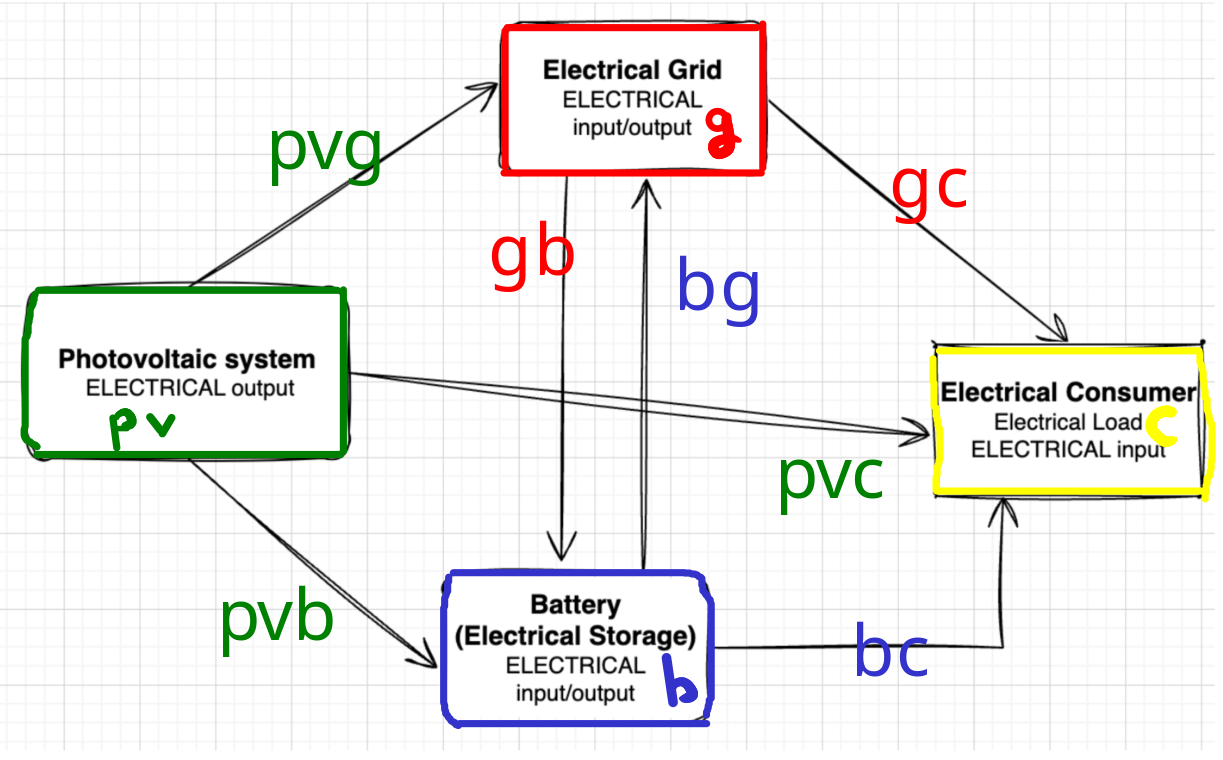
\includegraphics[width = \textwidth]{diagram}
\caption{The different flows that represent the variables}
\label{fig:diagram}
\end{figure}

\begin{itemize}
\item $\mathbf{pvg}_t$: Flow from photovoltaic system to grid at time $t$ (kW).
\item $\mathbf{pvc}_t$: Flow from photovoltaic system to consumer at time $t$ (kW).
\item $\mathbf{pvb}_t$: Flow from photovoltaic system to battery at time $t$ (kW).
\item $\mathbf{gb}_t$: Flow from the grid to battery at time $t$ (kW).
\item $\mathbf{gc}_t$: Flow from the grid to the consumer at time $t$ (kW).
\item $\mathbf{bg}_t$: Flow from the battery to the grid at time $t$ (kW).
\item $\mathbf{bc}_t$: Flow from the battery to the consumer at time $t$ (kW).
\item $\mathbf{charge}_t$: Charge level of the battery at time $t$ (kWh).
\end{itemize}

All the variables are nonnegative real values. See Figure \ref{fig:diagram}.

\subsection{Data}

\begin{itemize}
\item $\mathbf{pv}_t$: Predicted photovoltaic production at time $t$ (kW).
\item $\mathbf{conso}_t$: Predicted consumption at time $t$ (kW).
\item $\mathbf{lcos}_t$: Levelized cost of storage at time $t$ (cents/kWh).
\item $\mathbf{sell}_t$: Selling price of the energy at time $t$ (cents/kWh).
\item $\mathbf{buy}_t$: Buying price of the energy at time $t$ (cents/kWh).
\end{itemize}

\subsection{Objective Function}

\begin{equation}
\min C = \sum_t \mathbf{buy}_t \cdot \mathbf{eb}_t - \mathbf{sell}_t \cdot \mathbf{es}_t + \mathbf{lcos}_t \cdot \mathbf{ed}_t
\end{equation}

where:

\begin{itemize}
\item The bought energy $\mathbf{eb}_t = \mathbf{gb}_t + \mathbf{gc}_t$ is the sum of the grid to battery flow ($\mathbf{gb}_t$) and the grid to consumer flow ($\mathbf{gc}_t$).
\item The sold energy $\mathbf{es}_t = \mathbf{bg}_t + \mathbf{pvg}_t$ is the sum of the battery to grid flow ($\mathbf{bg}_t$) and the photovoltaic system to grid flow ($\mathbf{pvg}_t$).
\item The discharged energy $\mathbf{ed}_t = \mathbf{bc}_t + \mathbf{bg}_t$ is the sum of the battery to consumer flow ($\mathbf{bc}_t$) and the battery to grid flow ($\mathbf{bg}_t$).
\end{itemize}

\subsection{Constraints}

\textbf{Photovoltaic Production:}

\begin{equation}
\mathbf{pvg}_t + \mathbf{pvc}_t + \mathbf{pvb}_t \leq \mathbf{pv}_t \, , \quad \forall t
\end{equation}

\textbf{Battery:}

\begin{eqnarray}
\mathbf{charge}_t \leq 160 \, , \quad \forall t \\
\text{(Max discharge)} \quad \mathbf{bg}_t + \mathbf{bc}_t \leq 100 \, , \quad \forall t \\
\text{(Max charge)} \quad \mathbf{gb}_t + \mathbf{pvb}_t \leq 100 \, , \quad \forall t
\end{eqnarray}

Evolution of the level of charge in the battery:
\begin{equation}
\mathbf{charge}_t =
\begin{cases}
0.92 \cdot (\mathbf{gb}_t + \mathbf{pvb}_t) - (\mathbf{bg}_t + \mathbf{bc}_t) & \text{if } t = 0 \\
\mathbf{charge}_{t-1} + 0.92 \cdot (\mathbf{gb}_t + \mathbf{pvb}_t) - (\mathbf{bg}_t + \mathbf{bc}_t) & \text{if } t > 0
\end{cases}
\end{equation}

where the charging efficiency of the battery is $92 \%$.

\textbf{Grid:}

\begin{eqnarray}
\text{(Max sell power)} \quad \mathbf{bg}_t + \mathbf{pvg}_t \leq 700 \, , \quad \forall t \\
\text{(Max buy power)} \quad \mathbf{gb}_t + \mathbf{gc}_t \leq 700 \, , \quad \forall t
\end{eqnarray}

\textbf{Consumer Demands:}

\begin{equation}
\mathbf{gc}_t + \mathbf{pvc}_t + \mathbf{bc}_t = \mathbf{conso}_t \, , \quad \forall t
\end{equation}

\subsection{Results of the optimization}

See Figure \ref{fig:resultsPartA}.

\begin{figure}
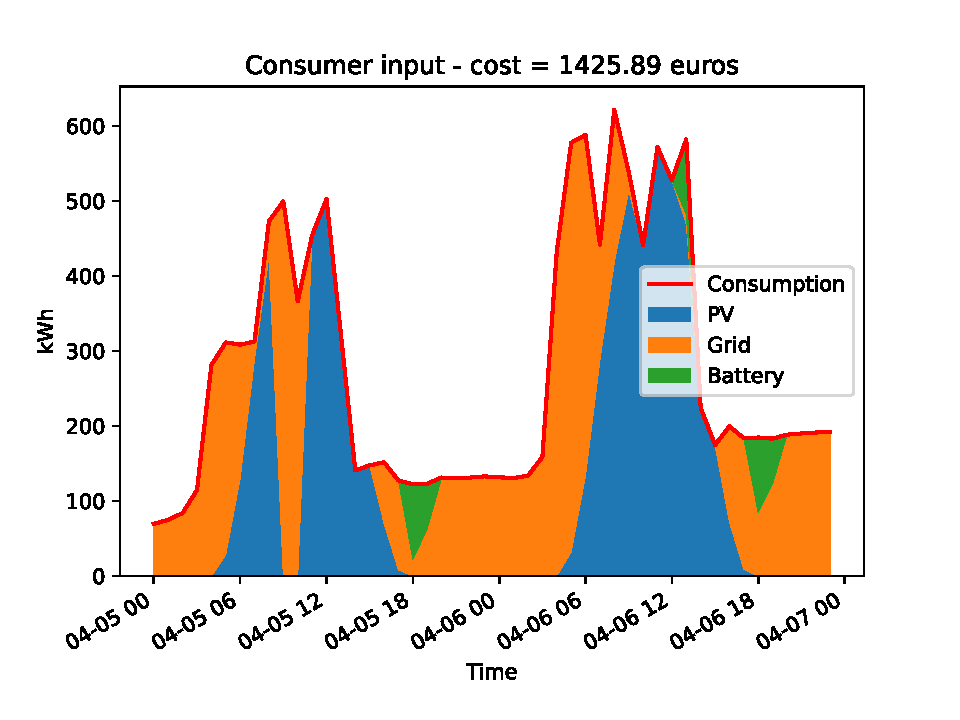
\includegraphics[width = \textwidth]{consumer_input}
\caption{Results of Part A of the example from \textit{test\_data.xlsx}}
\label{fig:resultsPartA}
\end{figure}

\section{Part B}

To prevent simultaneous buying and selling from the grid, we introduce two binary variables:

\begin{itemize}
\item $\mathbf{to\_buy}_t \in \{0, 1\}$: This binary variable indicates whether we are buying energy from the grid ($1$) or not ($0$) at time $t$.
\item $\mathbf{to\_sell}_t \in \{0, 1\}$: This binary variable indicates whether we are selling energy to the grid ($1$) or not ($0$) at time $t$.
\end{itemize}

We add a constraint to ensure that buying and selling do not occur at the same time:

\begin{equation}
\mathbf{to\_buy}_t + \mathbf{to\_sell}_t \leq 1 \, , \quad \forall t
\end{equation}

Additionally, we introduce two constraints (through the Big-M method) to enforce the effect of the binary variables on the energy flows:

\begin{eqnarray}
\mathbf{gb}_t + \mathbf{gc}_t \leq \mathbf{to\_buy}_t \cdot M \, , \quad \forall t \\
\mathbf{bg}_t + \mathbf{pvg}_t \leq \mathbf{to\_sell}_t \cdot M \, , \quad \forall t
\end{eqnarray}

where $M > 0$ is any large enough number (we took $M = 10^5$).

These constraints ensure that energy is only bought or sold when the corresponding binary variable is active.

The results of implementing these constraints are illustrated in Figures \ref{fig:resultsPartB} and \ref{fig:buy_or_sellPartB}.

\begin{figure}
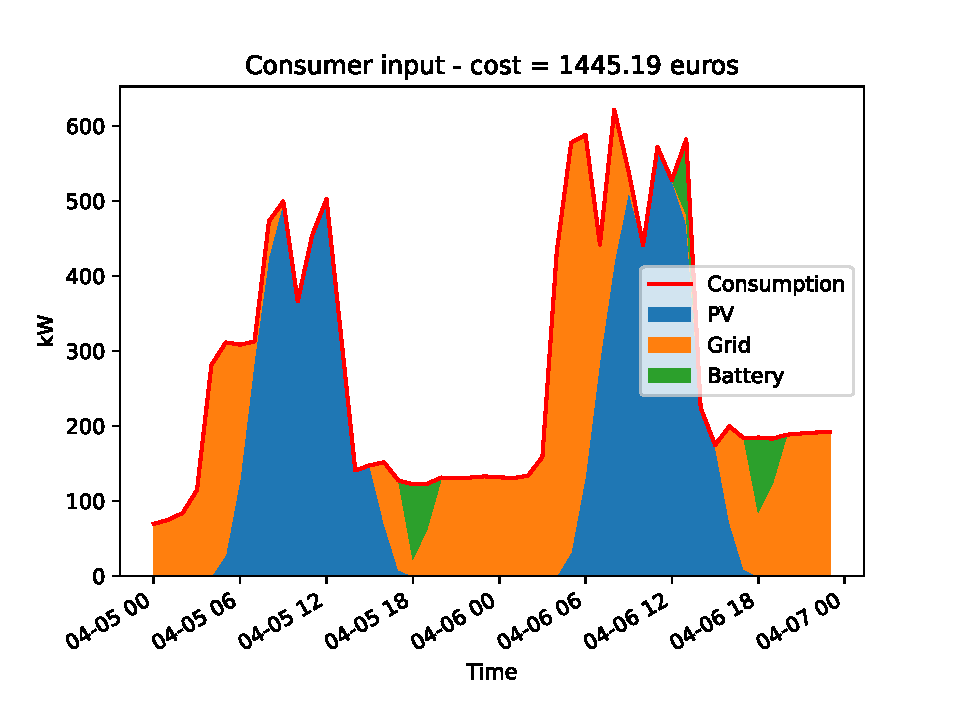
\includegraphics[width = \textwidth]{consumer_input_PartB}
\caption{Results of Part B of the example from \textit{test\_data.xlsx}}
\label{fig:resultsPartB}
\end{figure}

\begin{figure}
\includegraphics[width = \textwidth]{buy_or_sell_partB}
\caption{The amount of energy bought and sold over time (Part B). We do ensure that we do not buy and sell simultaneously.}
\label{fig:buy_or_sellPartB}
\end{figure}

\end{document}
